\documentclass[a4paper,12pt]{article}
\usepackage[utf8]{inputenc}
\usepackage[T1]{fontenc}
\usepackage{lmodern}
\usepackage{geometry}
\usepackage{setspace}
\usepackage{fancyhdr}
\usepackage{hyperref}
\usepackage{amsmath}
\usepackage{amsfonts}
\usepackage{amssymb}
\usepackage{mathtools}
\usepackage{float}
\usepackage{tabularx}
\usepackage{enumitem}
\usepackage{graphicx}
\usepackage{ragged2e}
\usepackage[spanish]{babel}
\usepackage{booktabs}
\usepackage{longtable}
\usepackage{multirow}
\usepackage{xcolor}
\usepackage{microtype}
\usepackage{caption}
\usepackage{textcomp}
\newcommand{\euro}{\texteuro}
\newcommand{\E}{\mathbb{E}}
\newcommand{\Var}{\mathrm{Var}}
\newcommand{\Cov}{\mathrm{Cov}}
\newcommand{\VaR}{\mathrm{VaR}}
\newcommand{\TVaR}{\mathrm{TVaR}}
\addto\captionsspanish{\renewcommand{\tablename}{Tabla}}
\addto\captionsspanish{\renewcommand{\figurename}{Figura}}
\captionsetup{font=small,labelfont=bf}

% Configuración de márgenes
\geometry{left=2.5cm,right=2.5cm,top=3cm,bottom=3cm}

% Configuración de encabezados y pies de página
\pagestyle{fancy}
\fancyhf{}
\renewcommand{\headrulewidth}{0pt}
\fancyfoot[C]{\thepage}

% Configuración de interlineado
\onehalfspacing
\justifying

% Configuración de hipervínculos
\hypersetup{
    hidelinks,
    colorlinks=false
}

\begin{document}

% Primera página (Título, Resumen y Abstract)
\begin{titlepage}
    \centering
    \vspace*{0.1cm}
    \huge\textbf{Tema 4: Preguntas de debate}\\
    \vspace{1cm}
    \small{Luiz Alberto Luzuriaga Izquierdo}\\
    \vspace{0.1cm}
    Facultad de ciencias económicas, empresariales y turismo. \\
    \vspace{0.1cm}
    Universidad de Alcalá de Henares. \\
    \vspace{0.1cm}
    Curso 2026-2027\\
    \vspace{0.5cm}

{\bfseries Resumen}

\vspace{0.1cm}
\noindent
\begin{justify}
Respuestas argumentadas a las preguntas de debate del tema, con cifras de los casos prácticos. Tema 4 (Gestión de capital y medidas coherentes de riesgo: VaR y TVaR): Axiomas de Artzner, subaditividad del TVaR frente al VaR y su aplicación en Solvencia II y Basilea.\\\\
\vspace{0.1cm}
\noindent
\textbf{Palabras clave}: VaR, TVaR, medidas coherentes, subaditividad, preguntas de debate.
\end{justify}
\begin{center}
    {\bfseries Abstract}
\end{center}
\vspace{0.1cm}
\noindent
\begin{justify}
Class work for Topic 4 of Actuarial Mathematics of Stability and Solvency of Insurance Activity: discussion questions with actuarial reasoning and numerical evidence.\\\\
\vspace{0.1cm}
\noindent
\textbf{Keywords}: VaR, TVaR, coherent risk measures, subadditivity, discussion questions.
\end{justify}

\end{titlepage}

% Índice
\newpage\pagenumbering{gobble}
\renewcommand{\contentsname}{Índice}
\newgeometry{left=4cm, right=4cm, top=3cm, bottom=2.5cm}
\tableofcontents

\restoregeometry
\newpage
\numberwithin{equation}{section}
\pagenumbering{arabic}
\setcounter{page}{1}

\section{Tema 4: Gestión de capital y medidas coherentes de riesgo: VaR y TVaR}
\label{sec:tema4debate}
\noindent
Respuestas argumentadas a las preguntas de debate del tema, con cifras de los casos prácticos. Material de referencia: diapositivas del Tema 4 (Prof. Hugo González Riera).

\subsection{Debate 1 -- ?`Por qu\'e Solvencia~II mantiene el VaR y la banca migr\'o al ES?}

\paragraph{Tesis.} No es solo tradici\'on regulatoria: el problema de las aseguradoras (datos escasos, horizonte anual, colas pesadas, calibraci\'on de toda la f\'ormula est\'andar) hace que las razones del VaR pesen m\'as en seguros que en banca, y las razones del ES pesen m\'as donde hay riesgo de cola catastr\'ofica.

\paragraph{A favor del ES / TVaR.}
\begin{itemize}[leftmargin=*,itemsep=1pt]
\item \textbf{Coherencia:} subaditividad para cualquier dependencia. En el ejemplo de cr\'edito (50 M\euro\ cada cartera, $q=1{,}5\%$, $p=98\%$), el VaR \emph{crea} 50 M\euro\ al consolidar (0+0 frente a 50), mientras el TVaR reduce el capital de 75 a 50,56 M\euro.
\item \textbf{Informaci\'on de cola}: con la Normal el TVaR exige $+12{,}3\%$ de capital; con una Log-normal de la misma media y varianza, $+16{,}1\%$; con una $t_4$ el cociente $\TVaR_{99,5}/\VaR_{99,5}$ es $1{,}13$.
\item \textbf{Evita la optimizaci\'on de cola} (ver debate~3 y~2).
\end{itemize}

\paragraph{A favor del VaR en seguros.}
\begin{enumerate}[leftmargin=*,itemsep=2pt]
\item \textbf{Datos.} Un banco usa series diarias de precios de mercado y horizonte de 10 d\'ias; una aseguradora tiene un dato por a\~no y una distribuci\'on a un a\~no con pasivos a decenios. En una simulaci\'on con una $t_4$, el error t\'ipico del ES al 99\,\% es mayor que el del VaR al 99,5\,\%: $25{,}2\%$ frente a $21{,}2\%$ con 250 observaciones; $10{,}6\%$ frente a $9{,}0\%$ con 2.000. Con una cola Pareto de $\alpha$ cercano a 1 el ES es enorme e inestable, y no existe con $\alpha\le1$.
\item \textbf{Contrastaci\'on.} El VaR es elicitable (se valida contando excesos); el ES s\'olo lo es conjuntamente con el VaR. El \emph{backtesting} del FRTB sigue haci\'endose sobre el VaR (al 99\,\%) y una validaci\'on del capital por ES es m\'as d\'ebil.
\item \textbf{Calibraci\'on.} La f\'ormula est\'andar, las correlaciones entre m\'odulos, el margen de riesgo y los modelos internos est\'an calibrados al VaR 99,5\,\%; cambiar la medida exige recalibrar todo y una transici\'on larga. Adem\'as, la ganancia no es tan grande si las marginales son casi normales: $\TVaR_{99\%}/\VaR_{99,5\%}=1{,}03$ con la Normal.
\item \textbf{Comparabilidad y comunicaci\'on.} Probabilidad de ruina del $0{,}5\%$ a un a\~no (rating BBB aproximado) es un mensaje directo al asegurado, al Consejo y al mercado. El \emph{Insurance Capital Standard} de la IAIS tambi\'en usa VaR 99,5\,\%.
\end{enumerate}

\paragraph{La diferencia entre sectores.} La banca (FRTB) tiene carteras de negociaci\'on valoradas a mercado, datos diarios, riesgo de cola de mercado muy observado en 2008 y horizontes de liquidez expl\'icitos (10--120 d\'ias). En seguros el riesgo catastr\'ofico y de longevidad es el que realmente vive en la cola, pero tiene muy pocas observaciones. Es un argumento \emph{a favor} del ES en materia de severidad (no se puede ignorar la cola), y \emph{en contra} en materia de estimaci\'on.

\paragraph{Un hecho que relativiza el debate.} Los dos niveles no son tan distintos en la pr\'actica: $\TVaR_{p'}=\VaR_{99,5\%}$ para $p'=98{,}7\%$ (Normal), $98{,}4\%$ ($t_4$) o $98{,}0\%$ (Pareto $\alpha=2$). La elecci\'on entre VaR 99,5\,\% y ES 99\,\% (SST) cambia el capital en torno al $3\%$ (Normal) y hasta el $41\%$ (Pareto $\alpha=2$) seg\'un la cola.

\paragraph{Conclusi\'on.} Mantener el VaR se justifica por datos, calibraci\'on y comparabilidad; migrar al ES, por coherencia y cola. La v\'ia razonable es un enfoque h\'ibrido: capital por VaR 99,5\,\%, m\'as informaci\'on de cola (TVaR) obligatoria en ORSA y modelos internos.

\bigskip\hrule\bigskip

\subsection{Debate 2 -- Mismo VaR al 99,5\,\%, distinta cola: ?`mismo capital?}

\paragraph{Tesis.} No. El VaR responde a ``?`cu\'anto pierdo en el percentil 99,5\,\%?'' y no a ``?`cu\'anto pierdo cuando lo supero?''. Dos carteras con el mismo VaR pueden ser radicalmente distintas.

\paragraph{Ejemplo construido.} Cartera $X\sim N(5;0{,}8^2)$ M\euro\ y cartera $Y$ con una componente normal $N(5;0{,}667^2)$ y, con probabilidad $0{,}4\%$ (menor que $1-p=0{,}5\%$), una p\'erdida catastr\'ofica de 30 M\euro. Se ajusta la parte normal para que ambas tengan el mismo $\VaR_{99,5}=7.060.663$ \euro:
\begin{center}
\small
\begin{tabular}{lrr}
\toprule
 & $X$ (Normal) & $Y$ (con catástrofe)\\
\midrule
$\E[S]$ & 5.000.000 & 5.100.000\\
$\VaR_{99\%}$ & 6.861.078 & 6.674.878\\
$\VaR_{99,5\%}$ & 7.060.663 & 7.060.663\\
$\VaR_{99,6\%}$ & 7.121.656 & 10.749.032\\
$\VaR_{99,9\%}$ & 7.472.186 & 30.000.000\\
$\TVaR_{99,5\%}$ & 7.313.559 & 25.449.081\\
\bottomrule
\end{tabular}
\end{center}
\begin{figure}[H]\centering
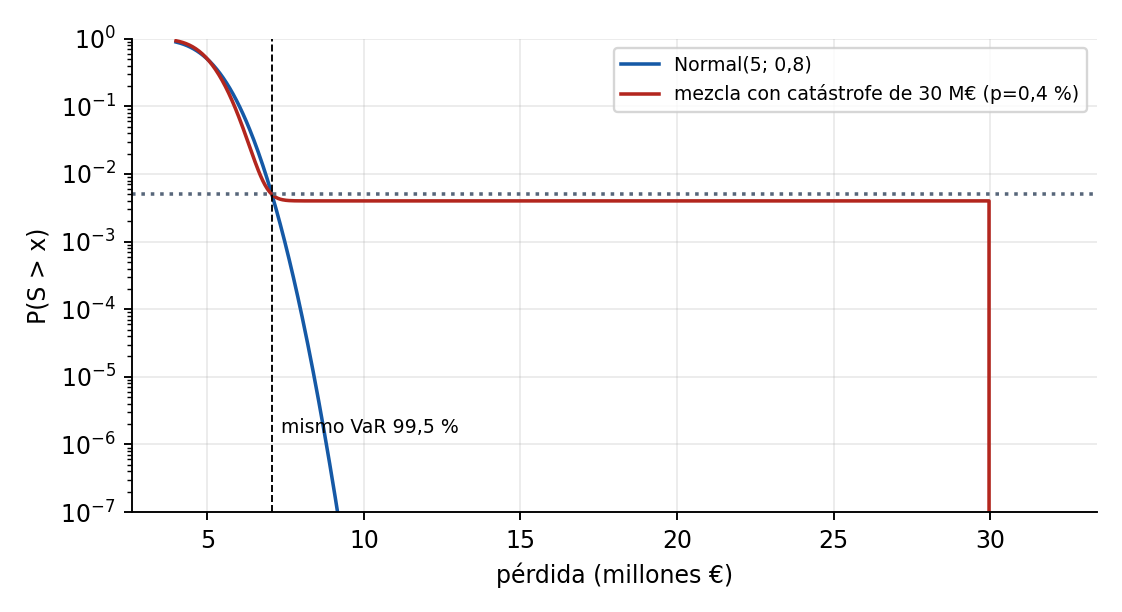
\includegraphics[width=.72\linewidth]{t4_f_debate2.png}
\caption{Colas de ambas carteras en escala logar\'itmica: el VaR al 99,5\,\% coincide, el comportamiento m\'as all\'a no.}
\end{figure}
El $\TVaR$ de $Y$ es $3{,}5$ veces el de $X$ ($25{,}4$ frente a $7{,}3$ M\euro), la media apenas cambia ($+2\%$) y el VaR al 99\,\% de $Y$ es \emph{menor} que el de $X$: un VaR a un solo nivel puede incluso favorecer a la cartera m\'as peligrosa. Un cambio de 0,1 puntos de $p$ (de 99,5 a 99,6\,\%) lleva el VaR de $Y$ de 7,06 a 10,75 M\euro.

\paragraph{Qu\'e capital deber\'ia exigirse.} Deber\'ian exigirse capitales distintos: el riesgo ``de verdad'' est\'a en la cola que el percentil no mira. Con una medida coherente sensible a la cola (TVaR/ES) el capital de $Y$ ser\'ia unas tres veces el de $X$.

\paragraph{M\'etricas y an\'alisis adicionales.}
\begin{itemize}[leftmargin=*,itemsep=1pt]
\item \textbf{TVaR/ES a varios niveles} (97,5, 99, 99,5, 99,9\,\%) y el \textbf{cociente TVaR/VaR} como alarma: en una Normal es $\approx1{,}04$; en $Y$, $3{,}5$.
\item \textbf{Curva VaR$_p$ en un rango de $p$}: la distancia entre VaR$_{99,5}$ y VaR$_{99,9}$ detecta saltos.
\item \textbf{\'Indice de cola} (Hill, EVT, Tema~5) y funci\'on de exceso medio: para una Pareto, $TVaR/VaR\to\alpha/(\alpha-1)$.
\item \textbf{Escenarios y \emph{stress tests}} extremos (catástrofe de 1 en 250, pandemia) y \textbf{pérdida máxima} contratada.
\item \textbf{Medidas espectrales} que ponderan m\'as la cola, o \textbf{distorsiones} (Wang).
\item \textbf{Reaseguro y exposici\'on neta} por encima del VaR: si hay una cobertura de cat\'astrofe, el TVaR neto puede ser razonable.
\end{itemize}

\paragraph{Conclusi\'on.} El capital deber\'ia reflejar la severidad de la cola; el VaR a un solo nivel es insuficiente y manipulable. Un buen marco combina un VaR regulatorio con medidas de cola y escenarios.

\bigskip\hrule\bigskip

\subsection{Debate 3 -- Riesgos de gobernanza si se usa el VaR para estructurar filiales}

\paragraph{Tesis.} Un VaR no subaditivo crea un incentivo de \emph{arbitraje regulatorio}: la estructura legal pasa a ser una palanca para reducir capital, no el reflejo del riesgo.

\paragraph{1. Fragmentaci\'on.} Sea un grupo con $n$ bonos independientes ($q=2\%$, p\'erdida 100) y $p=97{,}5\%$. Si cada bono se coloca en una filial, el capital por VaR es $0$ en cada una. Consolidado:
\begin{center}
\small
\begin{tabular}{rrrrr}
\toprule
$n$ bonos & VaR consolidado & $\sum$VaR por filial & TVaR consolidado & $\sum$TVaR por filial\\
\midrule
2 & 100 & 0 & 101,6 & 160\\
10 & 100 & 0 & 168,3 & 800\\
25 & 200 & 0 & 259,3 & 2.000\\
50 & 300 & 0 & 386,1 & 4.000\\
100 & 500 & 0 & 582,8 & 8.000\\
\bottomrule
\end{tabular}
\end{center}
Con VaR, repartir 100 bonos en 100 filiales hace que el capital exigido baje de $500$ a $0$ sin cambiar el riesgo ni un \'atomo. Con TVaR, el capital de la estructura fragmentada ($8.000$) es mayor que el consolidado ($582{,}8$): fragmentar nunca resulta rentable, la propiedad que se desea.

\paragraph{2. Optimizaci\'on de cola.} Tambi\'en se puede \emph{no} cambiar la estructura y s\'i el perfil: vender un riesgo con probabilidad por debajo de $1-p$ y p\'erdida enorme (por ejemplo, protecci\'on contra eventos extremos o garant\'ias de baja probabilidad) cobra prima y no toca el VaR. En el ejemplo de los bonos, a\~nadir una p\'erdida adicional del $0{,}4\%$ de probabilidad deja $\VaR_{97,5}=0$ pero sube el TVaR de $96$ a $256$ ($L=1.000$) y a $1.696$ ($L=10.000$). Es el mecanismo que se vio en 1998 (LTCM) y 2008: asumir riesgos que el VaR no ve.

\paragraph{3. Efectos sobre la gobernanza.}
\begin{itemize}[leftmargin=*,itemsep=1pt]
\item \textbf{Decisiones de estructura guiadas por el capital}, no por la estrategia: filiales, \emph{ring-fencing}, vehículos de titulización con el \'unico fin de bajar el VaR.
\item \textbf{Incentivos y retribuci\'on} ligados a rentabilidad sobre capital regulatorio (RoC) o RORAC: premia al directivo que reduce el VaR, no el riesgo.
\item \textbf{Informaci\'on enga\~nosa al Consejo y al supervisor:} el capital VaR transmite una diversificaci\'on o una seguridad inexistentes; se debilita el ORSA.
\item \textbf{Riesgo sistémico:} si muchas entidades fragmentan o ``optimizan la cola'' igual, el sistema acumula riesgo extremo invisible.
\item \textbf{Riesgo legal y reputacional} si el supervisor interpreta la estructura como elusi\'on.
\end{itemize}

\paragraph{4. C\'omo mitigarlo.}
\begin{itemize}[leftmargin=*,itemsep=1pt]
\item Medida coherente para el capital de grupo (o complementaria) y supervisi\'on \emph{de grupo} consolidada, con reglas de aplicaci\'on y de sustancia econ\'omica (T\'itulo~III de la Directiva 2009/138/CE, supervisi\'on de grupos).
\item Evaluaci\'on interna del riesgo (ORSA) con TVaR y escenarios; l\'imites de concentraci\'on en cola y de riesgos con baja probabilidad y alta severidad.
\item Retribuci\'on ajustada por riesgo de cola y diferimiento.
\item Prueba de \'uso (\emph{use test}) y validaci\'on independiente de la estructura de capital.
\end{itemize}

\paragraph{Conclusi\'on.} Con un VaR no subaditivo, el capital depende de la forma jur\'idica y de la cola oculta. El TVaR elimina el incentivo de fragmentar y reduce el de ocultar cola; el resto lo cubren la gobernanza y la supervisi\'on de grupo.

\bigskip\hrule\bigskip

\subsection{Debate 4 -- ?`Es razonable la homogeneidad positiva con posiciones grandes y poco l\'iquidas?}

\paragraph{Tesis.} No siempre. Duplicar una posici\'on grande e il\'iquida m\'as que duplica el riesgo, porque liquidarla cuesta m\'as por unidad. La respuesta de la literatura es \emph{relajar} la homogeneidad (y la subaditividad) y exigir solo \textbf{convexidad}.

\paragraph{Por qu\'e falla.} Homogeneidad: $\rho(\lambda X)=\lambda\rho(X)$. Si liquidar $\lambda$ unidades tiene un impacto en precio creciente (por ejemplo con coste cuadr\'atico $\kappa\lambda^2$), el riesgo efectivo es $\rho_{liq}(\lambda)=\lambda\rho+\kappa\lambda^2>\lambda\rho$. Con el Caso~1 ($\rho=\VaR-\E=2.060.663$ \euro) y un coste de liquidaci\'on del $5\%$ de $\rho$ a escala 1:
\begin{center}
\small
\begin{tabular}{rrrr}
\toprule
Escala $\lambda$ & $\lambda\rho$ & $\rho_{liq}(\lambda)=\lambda\rho+\kappa\lambda^2$ & $\rho_{liq}/(\lambda\rho)$\\
\midrule
1 & 2.060.663 & 2.163.696 & $105\%$\\
2 & 4.121.326 & 4.533.459 & $110\%$\\
5 & 10.303.315 & 12.879.144 & $125\%$\\
10 & 20.606.630 & 30.909.945 & $150\%$\\
\bottomrule
\end{tabular}
\end{center}
(Ilustrativo: el supuesto $\kappa=5\%\rho$ es una elecci\'on del ejercicio.) Es \emph{convexa} en $\lambda$ pero no homog\'enea.

\paragraph{La extensi\'on del marco de Artzner.}
\begin{itemize}[leftmargin=*,itemsep=2pt]
\item \textbf{Medidas de riesgo convexas} (F\"ollmer y Schied, 2002; Frittelli y Rosazza Gianin, 2002). Se sustituyen homogeneidad y subaditividad por \emph{convexidad} $\rho(\lambda X+(1-\lambda)Y)\le\lambda\rho(X)+(1-\lambda)\rho(Y)$, $\lambda\in[0,1]$: la diversificaci\'on sigue sin aumentar el riesgo, pero se admite que el riesgo crezca m\'as que proporcionalmente con el tama\~no.
\item \textbf{Medidas con liquidez} (Acerbi y Scandolo, 2008; Çetin, Jarrow y Protter, 2004): el valor de una cartera se define con el \emph{coste de liquidaci\'on} (curva de impacto de mercado) y el riesgo se mide sobre ese valor; la propiedad de homogeneidad se sustituye por una versi\'on que depende del tama\~no.
\item \textbf{Medidas entr\'opicas} $\rho_a(X)=\frac1a\ln\E[e^{aX}]$: convexas y no homog\'eneas. Con $X\sim N(\mu,\sigma^2)$, $\rho_a(\lambda X)=\lambda\mu+a\lambda^2\sigma^2/2$. Con $a=10^{-6}$ y el Caso~1: a escala 1, $5.320.000$; escala 2, $11.280.000$ frente a $2\rho_a(X)=10.640.000$ ($+6\%$); escala 10, $82.000.000$ frente a $53.200.000$ ($+54\%$). Es la utilidad exponencial del Tema~1 convertida en capital.
\end{itemize}

\paragraph{En la pr\'actica regulatoria.} El FRTB incorpora horizontes de liquidez diferenciados por factor de riesgo (de 10 a 120 d\'ias): el capital ES se escala por $\sqrt{(LH_j-LH_{j-1})/10}$ para tener en cuenta la dificultad de cerrar posiciones, lo que es una forma pragm\'atica de romper la homogeneidad. En seguros, las provisiones de liquidez, el margen de riesgo y los l\'imites de concentraci\'on cumplen la misma funci\'on.

\paragraph{Cu\'ando s\'i es razonable la homogeneidad.} Para riesgos de suscripci\'on diversificados y l\'iquidos de forma pr\'actica (no negociados), donde ``duplicar la cartera'' significa duplicar p\'olizas iguales con las mismas condiciones, y para un an\'alisis de primer orden. Pero hay efectos que la rompen: concentraci\'on, iliquidez de activos grandes, riesgo de reputaci\'on, capacidad de reaseguro limitada (el precio sube al aumentar la cesi\'on) y rendimientos de escala en gastos.

\paragraph{Conclusi\'on.} La homogeneidad es una simplificaci\'on \'util y un supuesto fuerte. La respuesta formal son las medidas convexas (con coste de liquidaci\'on); la pr\'actica del FRTB ya incorpora esa idea.

\subsubsection*{Referencias}
\begin{itemize}[leftmargin=*,itemsep=0pt]
\item Artzner, P., Delbaen, F., Eber, J.-M. y Heath, D. (1999). Coherent measures of risk. \emph{Mathematical Finance}, 9(3).
\item F\"ollmer, H. y Schied, A. (2002). Convex measures of risk and trading constraints. \emph{Finance and Stochastics}, 6.
\item Frittelli, M. y Rosazza Gianin, E. (2002). Putting order in risk measures. \emph{Journal of Banking \& Finance}, 26.
\item Acerbi, C. y Scandolo, G. (2008). Liquidity risk theory and coherent measures of risk. \emph{Quantitative Finance}, 8(7).
\item McNeil, A. J., Frey, R. y Embrechts, P. \emph{Quantitative Risk Management}. Princeton University Press.
\item Basel Committee on Banking Supervision (2016). \emph{Minimum capital requirements for market risk}.
\end{itemize}

\end{document}
